\documentclass[12pt, twoside, openright]{report} % Fuente a 12pt, formato doble página y chapter a la derecha
\raggedbottom % No ajustar el contenido con un salto de página

% MÁRGENES: 2,5 cm sup. e inf.; 3 cm izdo. y dcho.
\usepackage[
a4paper,
vmargin=2.5cm,
hmargin=3cm
]{geometry}

% INTERLINEADO: Estrecho (6 ptos./interlineado 1,15) o Moderado (6 ptos./interlineado 1,5)
\renewcommand{\baselinestretch}{1.15}
\parskip=6pt

% DEFINICIÓN DE COLORES para portada y listados de código
\usepackage[table]{xcolor}
\definecolor{azulUC3M}{RGB}{0,0,102}
\definecolor{gray97}{gray}{.97}
\definecolor{gray75}{gray}{.75}
\definecolor{gray45}{gray}{.45}

% Soporte para GENERAR PDF/A
\usepackage{etoolbox}
\makeatletter
\@ifl@t@r\fmtversion{2021-06-01}%
 {\AddToHook{package/after/xmpincl}
   {\patchcmd\mcs@xmpincl@patchFile{\if\par}{\ifx\par}{}{\fail}}}{}
\makeatother
\usepackage[a-1b]{pdfx}

% ENLACES
\usepackage{hyperref}
\hypersetup{colorlinks=true,
  linkcolor=black, % enlaces a partes del documento (p.e. índice) en color negro
  urlcolor=blue} % enlaces a recursos fuera del documento en azul

% Añadir pdfs como partes del documento
\usepackage{pdfpages}

% Quitar la indentación de principio de los párrafos
\setlength{\parindent}{0em}

% EXPRESIONES MATEMÁTICAS
\usepackage{amsmath,amssymb,amsfonts,amsthm}

\usepackage{txfonts} 
\usepackage[T1]{fontenc}
\usepackage[utf8]{inputenc}

% Insertar gráficas y fotos
\usepackage{tikz}
\usepackage{pgfplots}

\usepackage[spanish, es-tabla]{babel} 
\usepackage[babel, spanish=spanish]{csquotes}
\AtBeginEnvironment{quote}{\small}

% diseño de PIE DE PÁGINA
\usepackage{fancyhdr}
\pagestyle{fancy}
\fancyhf{}
\renewcommand{\headrulewidth}{0pt}
\fancyfoot[LE,RO]{\thepage}
\fancypagestyle{plain}{\pagestyle{fancy}}

% DISEÑO DE LOS TÍTULOS de las partes del trabajo (capítulos y epígrafes o subcapítulos)
\usepackage{titlesec}
\usepackage{titletoc}
\titleformat{\chapter}[block]
{\large\bfseries\filcenter}
{\thechapter.}
{5pt}
{\MakeUppercase}
{}
\titlespacing{\chapter}{0pt}{0pt}{*3}
\titlecontents{chapter}
[0pt]                                               
{}
{\contentsmargin{0pt}\thecontentslabel.\enspace\uppercase}
{\contentsmargin{0pt}\uppercase}                        
{\titlerule*[.7pc]{.}\contentspage}                 

\titleformat{\section}
{\bfseries}
{\thesection.}
{5pt}
{}
\titlecontents{section}
[5pt]                                               
{}
{\contentsmargin{0pt}\thecontentslabel.\enspace}
{\contentsmargin{0pt}}
{\titlerule*[.7pc]{.}\contentspage}

\titleformat{\subsection}
{\normalsize\bfseries}
{\thesubsection.}
{5pt}
{}
\titlecontents{subsection}
[10pt]                                               
{}
{\contentsmargin{0pt}                          
  \thecontentslabel.\enspace}
{\contentsmargin{0pt}}                        
{\titlerule*[.7pc]{.}\contentspage}  

% DISEÑO DE TABLAS.
\usepackage{multirow} % permite combinar celdas 
\usepackage{caption} % para personalizar el título de tablas y figuras
\usepackage{floatrow} % utilizamos este paquete y sus macros \ttabbox y \ffigbox para alinear los nombres de tablas y figuras de acuerdo con el estilo definido. Para su uso ver archivo de ejemplo 
\usepackage{array} % con este paquete podemos definir en la siguiente línea un nuevo tipo de columna para tablas: ancho personalizado y contenido centrado
\newcolumntype{P}[1]{>{\centering\arraybackslash}p{#1}}
\DeclareCaptionFormat{upper}{#1#2\uppercase{#3}\par}

% Diseño de tabla para ingeniería
\captionsetup[table]{
  format=hang,
  name=Tabla,
  justification=centering,
  labelsep=colon,
  width=.75\linewidth,
  labelfont=small,
  font=small,
}

% DISEÑO DE FIGURAS.
\usepackage{graphicx}
\graphicspath{{img/}} %ruta a la carpeta de imágenes

% Diseño de figuras para ingeniería
\captionsetup[figure]{
  format=hang,
  name=Fig.,
  singlelinecheck=off,
  labelsep=colon,
  labelfont=small,
  font=small    
}

% NOTAS A PIE DE PÁGINA
\usepackage{chngcntr} % Para numeración continua de las notas al pie
\counterwithout{footnote}{chapter}

% LISTADOS DE CÓDIGO
% soporte y estilo para listados de código. Más información en https://es.wikibooks.org/wiki/Manual_de_LaTeX/Listados_de_código/Listados_con_listings
\usepackage{listings}

% definimos un estilo de listings
\lstdefinestyle{estilo}{ frame=Ltb,
  framerule=0pt,
  aboveskip=0.5cm,
  framextopmargin=3pt,
  framexbottommargin=3pt,
  framexleftmargin=0.4cm,
  framesep=0pt,
  rulesep=.4pt,
  backgroundcolor=\color{gray97},
  rulesepcolor=\color{black},
  %
  basicstyle=\ttfamily\footnotesize,
  keywordstyle=\bfseries,
  stringstyle=\ttfamily,
  showstringspaces = false,
  commentstyle=\color{gray45},     
  %
  numbers=left,
  numbersep=15pt,
  numberstyle=\tiny,
  numberfirstline = false,
  breaklines=true,
  xleftmargin=\parindent
}

\captionsetup[lstlisting]{font=small, labelsep=period}
% fijamos el estilo a utilizar 
\lstset{style=estilo}
\renewcommand{\lstlistingname}{\uppercase{Código}}

\pgfplotsset{compat=1.17} 
%-------------
% DOCUMENTO
%-------------

\begin{document}
\pagenumbering{roman} % Se utilizan cifras romanas en la numeración de las páginas previas al cuerpo del trabajo

%----------
% PORTADA
%---------- 
\begin{titlepage}
	\begin{sffamily}
		\color{azulUC3M}
		\begin{center}
			\begin{figure}[H] % Incluimos el logotipo de la Universidad
				\makebox[\textwidth][c]{
\includegraphics[width=16cm]{Portada_Logo.png}}
			\end{figure}
			\vspace{2.5cm}
			\begin{Large}
				Grado en Ingeniería Informática\\
				2021-2022\\
				\vspace{2cm}
				\textsl{Apuntes}\\
				\bigskip
			\end{Large}
			{\Huge Inteligencia Artificial en las Organizaciones}\\
			\vspace*{0.5cm}
			\rule{10.5cm}{0.1mm}\\
			\vspace*{0.9cm}
			{\LARGE Jorge Rodríguez Fraile\footnote{\href{mailto:100405951@alumnos.uc3m.es}{Universidad: 100405951@alumnos.uc3m.es}  |  \href{mailto:jrf1616@gmail.com}{Personal: jrf1616@gmail.com}}}\\
			\vspace*{1cm}
		\end{center}
		\vfill
		\color{black}
		
\includegraphics[width=4.2cm]{img/creativecommons.png}\\
		Esta obra se encuentra sujeta a la licencia Creative Commons\\ \textbf{Reconocimiento - No Comercial - Sin Obra Derivada}
	\end{sffamily}
\end{titlepage}

%----------
% ÍNDICES
%---------- 

%--
% Índice general
%-
\tableofcontents
\thispagestyle{fancy}

%--
% Índice de figuras. Si no se incluyen, comenta las líneas siguientes
%-
\listoffigures
\thispagestyle{fancy}

%--
% Índice de tablas. Si no se incluyen, comenta las líneas siguientes
%-
\listoftables
\thispagestyle{fancy}

%----------
% TRABAJO
%---------- 

\pagenumbering{arabic} % numeración con números arábigos para el resto de la publicación  


%----------
% COMENZAR A ESCRIBIR AQUÍ
%---------- 

\chapter{Información}

\section{Profesores}
\begin{quote}
	Magistral: Agapito Ledesma, ledezma@inf.uc3m.es, solicitar tutorías por mail con antelación.

	Prácticas: Ascensión López Vargas, aslopezv@inf.uc3m.es.
\end{quote}

\chapter{Tema 0: Presentación}

\textbf{Películas sobre IA:} A.I. (Stephen Spielberg), I robot, Terminator (1984) y Morgan (2016).

Sophia, robot social.

Lo que tiene YouTube es datos infinitos, miles de horas por segundo.
WhatsApp hecha para ser comprada al tener todo el nicho de mercado sobre los sistemas de comunicación y “gratis”.
La línea ética es fina en muchas ocasiones, toman muchos datos. La banca y aseguradoras se están beneficiando de la IA para ajustarse o predecir.

GIGO $\rightarrow$ Garbage In Garbage Out (es muy importante la calidad de los datos)

Con el COVID se trató de desarrollar modelos de IA, pero no se tenían apenas datos y menos de calidad.

\section{Tipos:}
\begin{itemize}
	\item Sistemas expertos/difusos, no es uno u otro, sino puntos intermedios. Discursos como poco o mucho.
	\item Redes de neuronas artificiales.
	\item Computación evolutiva, supervivencia del más capaz.
	\item Minoría de datos.
	\item Agentes inteligentes.
	\item Sistemas híbridos.
\end{itemize}

\section{Metodología:}
\begin{itemize}
	\item SPOC (Small Private Online Classes) $\rightarrow$ Teoría
	      \begin{itemize}
		      \item Del tema 2-9
		      \item Videos y lecturas complementarias.
		      \item Test de autoevaluación que se publicaran semanalmente sobre el temario visto.
	      \end{itemize}
	\item Magistral $\rightarrow$ Dudas, Casos prácticos y Test (Wooclap)
	\item Práctica
\end{itemize}

\section{Evaluación}
\begin{itemize}
	\item 60 \% Teoría, nota mínima 4.
	      \begin{itemize}
		      \item 30 \% 2 PEC
		            \begin{itemize}
			            \item Glosario de términos dados en las magistrales
			            \item Preguntas bibliografía
		            \end{itemize}
		      \item 10 \% Seminarios
		            \begin{itemize}
			            \item Presentación
			            \item Memoria
			            \item Coordinación grupal
			            \item Evaluación
		            \end{itemize}
		      \item 10 \% SPOC
		      \item 10 \% i-test en Wooclap
	      \end{itemize}
	\item 40 \% Práctica
	      \begin{itemize}
		      \item 15 \% Prácticas cortas.
		      \item 10 \% PEC prácticas.
		      \item 15 \% Práctica final.
	      \end{itemize}

\end{itemize}

\chapter{Tema 1: Introducción}
\section{Previa}
\subsection{Sistemas inteligentes}
Programas capaces de tomar decisiones, aprender, trabajar de manera autónoma, etc. Hubo un momento que era una palabra comodín, se utilizaba para atraer a la gente al producto, ¿pero realmente lo eran?

\subsection{Inteligencia}
Capacidad de entender, razonar y resolver problemas. Conocimiento, comprensión, acto de entender.

Howard Gardner publicó en 1983 la Teoría de las Inteligencias Múltiples, donde se exponía que no solo hay una manera de inteligencia, sino que dependiendo del ámbito hay un tipo de inteligencia especifica.
\begin{figure}[H]
	\ffigbox[\FBwidth]
	{\caption{Diagrama Inteligencias múltiples}}
	{\def\svgwidth{.8\textwidth}
		\input{img/inteligencia-multiple.eps_tex}}
\end{figure}

\subsection{Inteligencia Artificial}
\subsubsection{Definiciones}
Es una tecnología que parece emular el desempeño humano, típicamente aprendiendo, llegando a sus propias conclusiones, aparentando comprender contenido complejo, participando en diálogos naturales con personas, mejorando el desempeño  cognitivo humano o reemplazando personas en la ejecución de tareas no rutinarias.

Disciplina científica que se ocupa de crear programas informáticos que ejecutan operaciones comparables a las que realiza la mente humana, como el aprendizaje o el razonamiento lógico.

La IA no solo es el Deep Learning (Redes de neuronas), sino que hay multitud de áreas.
\begin{figure}[H]
	\ffigbox[\FBwidth]
	{\caption{Mapa de tecnologías IA}}
	{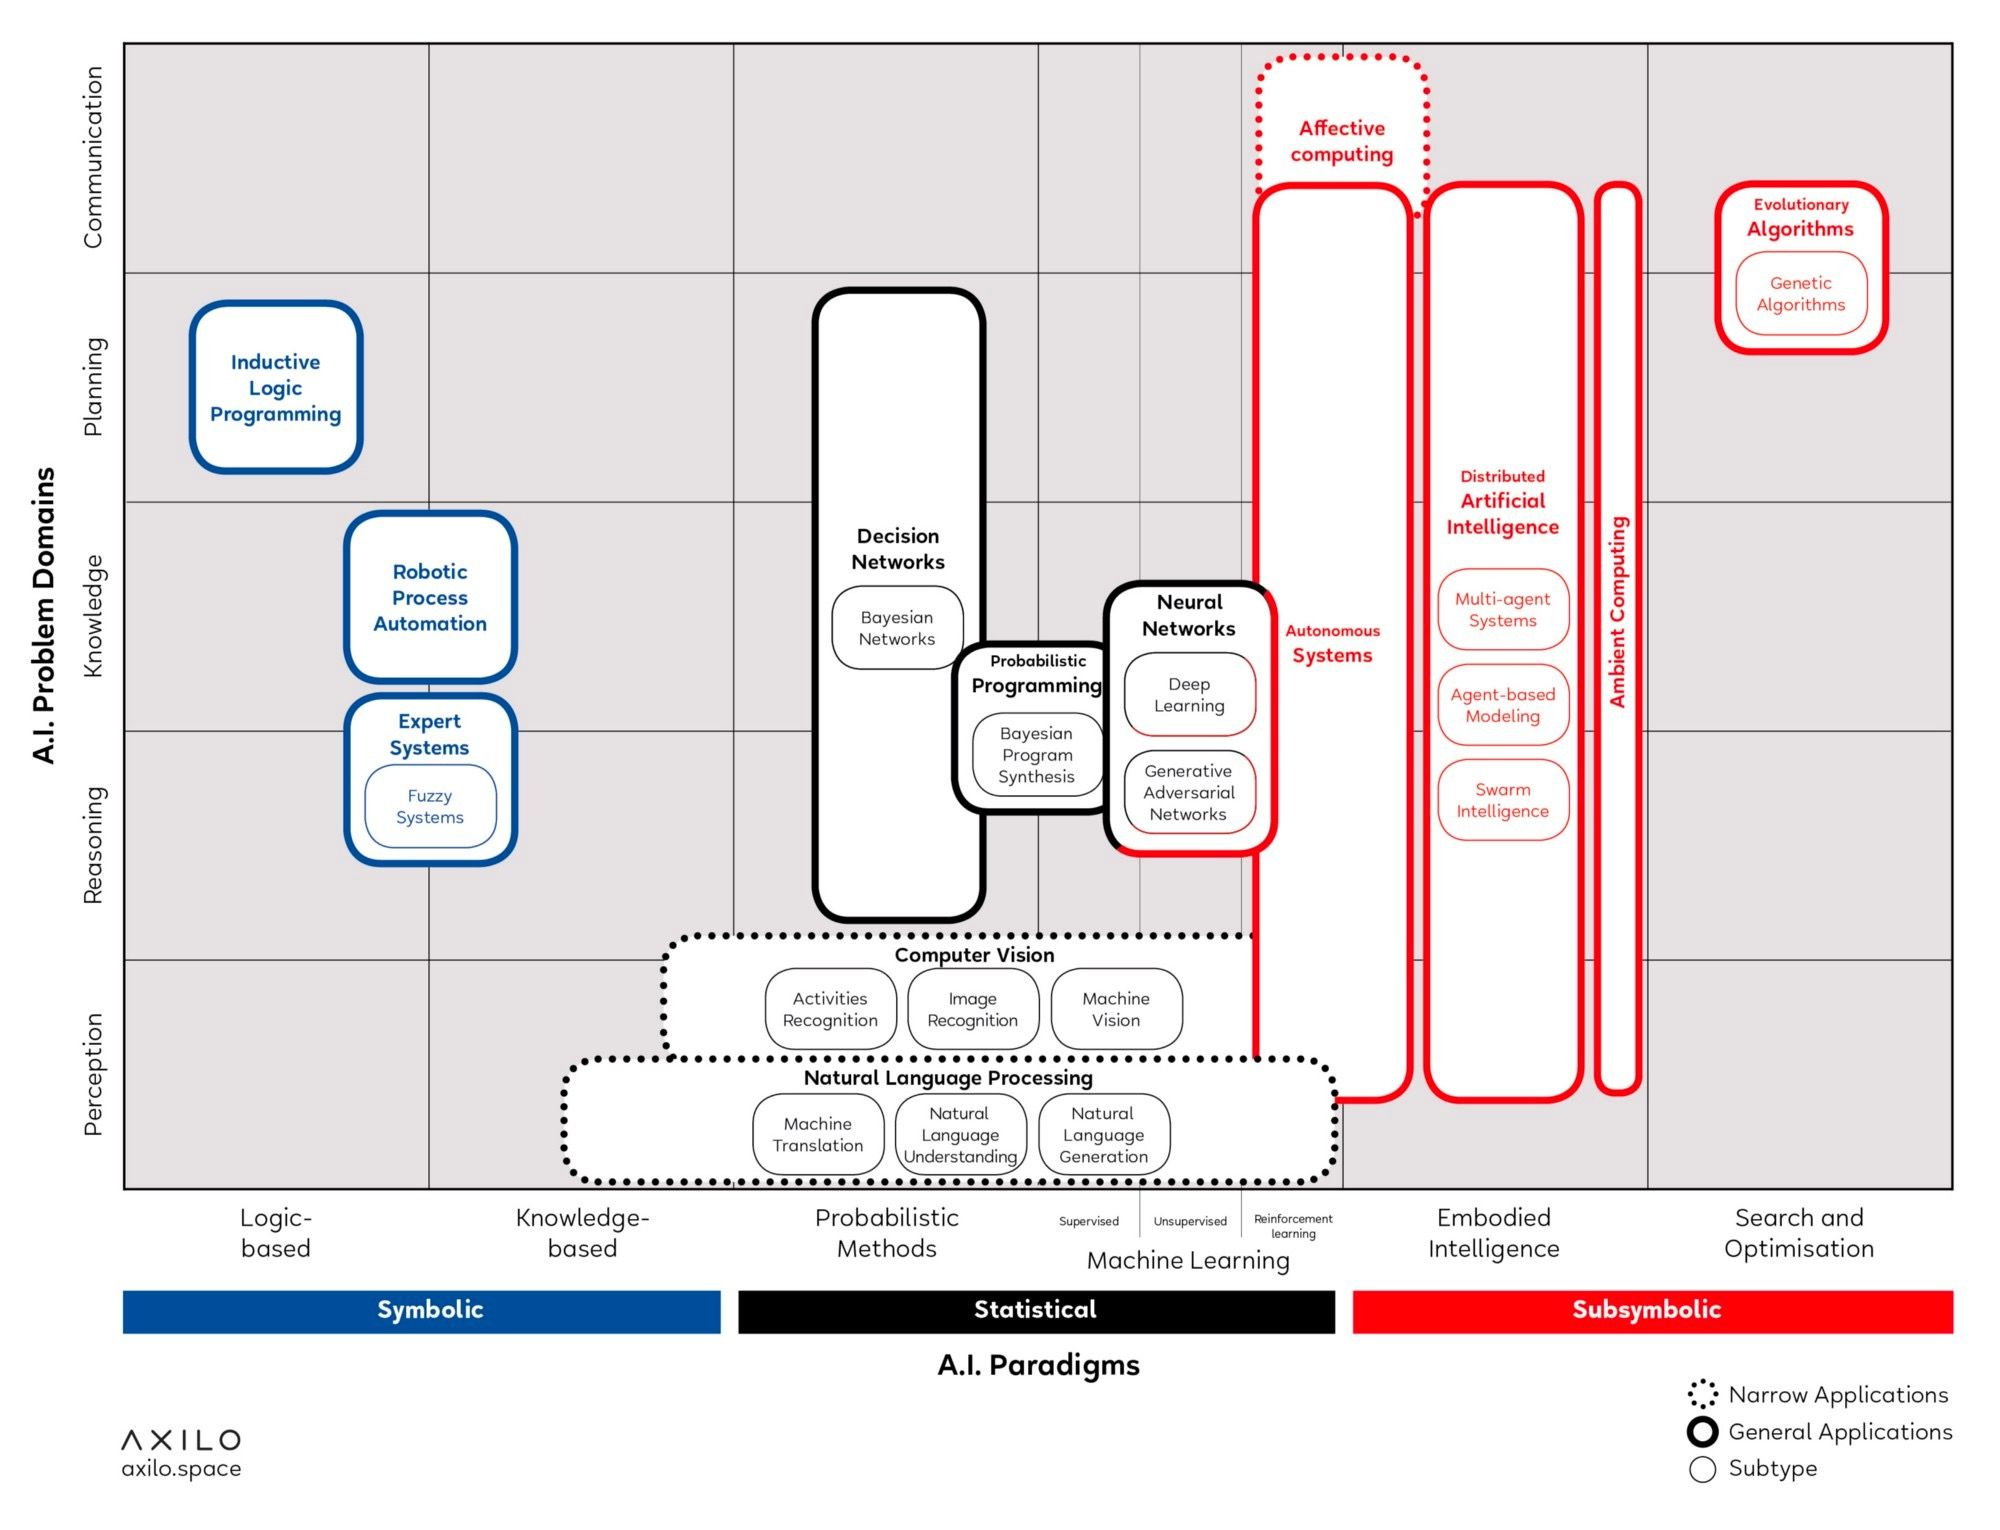
\includegraphics[scale=.23]{areas-ia.jpg}}
\end{figure}

\subsubsection{Historia}
El gran sueño del hombre ha sido siempre crear vida, por lo que hay multitud de proyectos para recrearla en forma de robots como son los geminoids. El problema con los robots que se parecen a los humanos no son sus formas humanoides, sino sus rasgos humanos que provocan del Valle inquietante (provocan incomodidad a las personas).

Por otro lado no solo se trata de que tengan la forma sino también que se comporten como personas, es decir que sean capaces de resolver los problemas de manera parecida siguiendo un razonamiento, de ahí la Inteligencia Artificial.

Alan Turing en 1950 antes de que se acuñase el término de IA dijo:
\begin{displayquote}
	Propongo considerar la siguiente cuestión: ¿pueden pensar las máquinas?
\end{displayquote}

En la cultura popular, literatura y el cine, se ha tratado este tema muchas veces como en Frankenstein, Matrix o Terminator.

En la realidad no hay nada que se parezca a un cerebro humano estamos muy lejos todavía de lograrlo, pero nos permite resolver ciertos problemas. Por ejemplo: Deep Blue de IBM, la RoboCup o Watson de IBM.

Estos últimos tiempos ha podido avanzar tan rápido gracias a la capacidad de cómputo (hardware) y la inmensa cantidad de datos que hay digitalizados y se generan por segundo.

Se han hecho estudios de cuánto tiempo tardará la IA en ser capaz de reemplazar al ser humano en determinadas tareas, como escribir un best-seller, ser cirujano o vendedor de tienda.

\subsection{Ejemplos de su uso}
\begin{itemize}
	\item Google Maps para estimar el tiempo de viaje.
	\item Filtros anti-spam buscando patrones similares a los clasificados como correo basura.
	\item Asistentes como Siri, Alexa o Cortana, eso vienen con un pre-aprendizaje para evitar sesgo.
	\item Antivirus busca patrones de comportamiento.
	\item Reconocimiento facial como en Facebook, Fotos iOS o Google Fotos.
	\item Drones repartidores para suplir la ‘last mile’, capaces de llevar cargas de un punto a otro y recargarse solos.
	\item Sistemas de recomendaciones según el comportamiento del usuario aprende sus gustos.
\end{itemize}

\subsection{Sectores que han adoptado IA mejor}
\begin{itemize}
	\item Alta tecnología y telecomunicaciones.
	\item Automovilística y ensamblado.
	\item Servicios financieros.
	\item Recursos y utilidades.
	\item Entretenimiento y media.
\end{itemize}

\section{Introducción}
En la actualidad se hace algo parecido al clásico ‘Artis Auriferae quam Chemiam vocant’ de la alquimia (química), que quiere decir El Arte de Hacer Oro que era la piedra filosofal de estos expertos, lo que les da poder.

Los profesionales de todas las áreas de la industria y los negocios buscan su particular piedra filosofal, en la actualidad el material valioso es el Conocimiento y el proceso es saber transformar los datos en conocimiento.

Los procesos que emplean los profesionales de negocios son Sistemas Inteligentes que buscan patrones no lineales, son de este tipo porque la mayoría de los problemas son de este tipo. Otro punto que hace complicado encontrar patrones y relaciones en los datos es que los que se encuentren sean útiles.

\subsection{Usos}
\begin{itemize}
	\item Predicción del comportamiento del consumidor, saber que consumen los clientes para de esta manera poder captar su atención y ofrecerles oferta o productos determinados. Actualmente los usuarios buscan un producto más personalizado.
	\item Captura del conocimiento corporativo, recogen el conocimiento de profesionales con experiencia para desarrollar un sistema experto que sea capaces de realizar sus tareas.
	\item Agricultura de precisión, para optimizar el regadío, los fertilizantes o abonos, de esta manera maximizar la producción y agricultura sostenible. Se emplean robots como Wall-Ye que toma medidas de la tierra.
	\item Detección de fraudes, permiten detectar si el usuario se está saliendo de su patrón de comportamiento (conocido por todas sus transacciones), levantar una alerta y bloquear el pago.

	      El factor más importante para combatir el fraude es el Tiempo, por lo que las RNA son una gran herramienta, son capaces de detectar patrones mucho más rápido que una persona y tiene la capacidad de adaptarse.
\end{itemize}
\pagebreak

\section{Contexto}
Todo hoy en día deja un rastro de datos, incluso aunque nosotros no llevemos dispositivos electrónicos hay cámaras, tarjetas, entre muchos otros que son capaces de recoger datos sobre nosotros.

Las grandes empresas (automotrices y financieras) fueron los primeros en darse cuenta de que esos datos son un gran activo que explotar. Los sistemas inteligentes que utilizan buscan relaciones y patrones en grandes cantidades de datos para extraer conocimiento.

Las técnicas más comunes son las Redes de Neuronas dado que hay muchas formas de estas, Algoritmos Genéticos y la lógica difusa. Antes se utilizaba en sistemas no principales, pero hoy en día en el núcleo de la empresa ‘core-business’.

Muchas de estas técnicas están inspiradas en la naturaleza (bioinspiradas), las redes de neuronas en el cerebro, algoritmo evolutivos o inteligencia de enjambre. La pregunta es si ha funcionado en la naturaleza porque no imitarlo para resolver otros problemas.

\subsection{Donde se usa}
\begin{itemize}
	\item \textbf{Banca al por menor:} Evaluación de hipotecas y Predicción de demanda de productos.
	\item \textbf{Planificación:} Localización de minoristas y Distribución de productos.
	\item \textbf{Seguros:} Evaluación de riesgos y Cálculo de primas.
	\item \textbf{Marketing:} Perfiles de clientes y Venta cruzada.
	\item \textbf{Banca de Inversiones:} Predicción de activos y Gestión de cartera.
	\item \textbf{Vigilancia:} Detección de robos internos y Detección de fraudes con tarjetas de crédito.
\end{itemize}

\subsection{Motivación}
Las empresas buscan la reducción de costes, aumentar la calidad del servicio y mejora de las prestaciones del producto.

\subsection{Redes de Neuronas Artificiales}
Es una simplificación de cómo funciona el cerebro humano, su objetivo no es simular el cerebro.

Es un array de números (pesos), que dada una entrada procesa los datos y produce una salida.

\subsection{Algoritmos evolutivos}
Se codifica la solución de un problema y se genera una serie de soluciones que no tienen por qué ser buenas, solo soluciones. Después estas soluciones se mutan para dar lugar a nuevas soluciones que se evaluaran con una función para quedarnos con las mejores, el proceso ser repite mejorando las soluciones progresivamente hasta llegar a la más cercana a la óptima (cuasi óptima).

Están muy orientadas a problemas de optimización.

\section{Características clave}
\begin{itemize}
	\item \textbf{Aprendizaje:} Es la característica más importante de los sistemas inteligentes. Las técnicas actuales difieren mucho de los primeros sistemas expertos, que tenían muy poca capacidad de aprender.
	\item \textbf{Adaptación:} Como todos los negocios y empresas cambian continuamente, los procesos se van quedando obsoletos, por lo que las técnicas tienen que ir evolucionando para seguir siendo útiles. Se podría reentrenar, no dejar de aprender o combinando dos procesos.
	\item \textbf{Flexibilidad:} Las decisiones humanas se caracterizan por una inherente flexibilidad, cada uno percibe las cosas de una manera distinta, pero todos lo hacemos dentro de un rango. Otra manera de expresarla es aun faltando un dato ser capaz de continuar y llevar a cabo el proceso. Los sistemas clásicos funcionan con lógica si/no.
	\item \textbf{Explicación:} Se debe saber cómo se llega a la conclusión del proceso, para poder entender como los realiza y esto permite la interacción el experto que sabrá si lo ha hecho bien. No te fiarías de una máquina que no sabes por qué dice que te tienes que operar.
	\item \textbf{Descubrimiento:} Capacidad de descubrir procesos o relaciones nuevas que no eran conocidas previamente.

	      Los patrones descubiertos deben ser validados por un experto humano.
\end{itemize}

\section{Principales técnicas}
\begin{table}[H]
	\centering
	\caption{Comparativa técnicas IA}
	\resizebox{\textwidth}{!}{%
		\begin{tabular}{|c|c|c|c|c|c|}
			\hline
			Técnica                    & Aprendizaje & Flexibilidad & Adaptación & Explicación                & Descubrimiento \\ \hline
			\begin{tabular}[c]{@{}c@{}}Redes de\\ Neuronas\end{tabular} & ↑↑↑↑↑       & ↑↑↑↑↑        & ↑↑↑↑↑      & \begin{tabular}[c]{@{}c@{}}↑ \\ Suelen ser\\ cajas negras\end{tabular} & ↑↑             \\ \hline
			\begin{tabular}[c]{@{}c@{}}Algoritmos\\ Genéticos\end{tabular} & ↑↑↑↑↑       & ↑↑↑↑         & ↑↑↑↑       & ↑↑↑                        & ↑↑↑↑↑          \\ \hline
			\begin{tabular}[c]{@{}c@{}}Sistemas \\ Borrosos\\ Fuzzy\end{tabular} & ↑           & ↑↑↑↑↑        & ↑          & ↑↑↑                        & ↑              \\ \hline
			\begin{tabular}[c]{@{}c@{}}Sistemas\\ Expertos\end{tabular} & ↑           & ↑            & ↑          & \begin{tabular}[c]{@{}c@{}}↑↑↑↑↑\\ Al estar basado\\ en reglas\end{tabular} & ↑              \\ \hline
		\end{tabular}%
	}
\end{table}
También existen técnicas híbridas.

\section{Actualidad}
La Inteligencia Artificial no reemplaza a las técnicas tradicionales, pero si las enriquece o presenta alternativas.

Algunos sistemas inteligentes producen salidas que pueden ser entendidas por los que toman las decisiones.

La tendencia actual es incorporar los sistemas inteligentes dentro de otras aplicaciones de negocios, actualmente es muy accesible, pero se necesita personal. Utilización en pequeñas y medianas empresas.

Los sistemas híbridos es un área en expansión.


\end{document}